\chapter{Arithmetic of a Deep Neural Network}\label{Chapter5}
\section {Digit Recognition Problem}
The MNIST data set is a set of images $28\times 28$ size of handwritten digits from 0-9 of which about 10000 are for testing the network and 60000 are for training the network.
Lenet 5 is a model designed for classification and recognition of images.
Convolutional Layer and max pool layer are two important features of the lenet family of models.
The implementation supported in [\ref{papaa}] is a working opencl implementation of lenet 5 model to classify the digits in MNIST data set. Also it has many labs to analyze the performance for CPU and GPU.
\subsection{Detailed Explanation of the Implementation}
The current library uses OPENCV which is a library written in C++ developed for computer vision applications. The entire implementation used 32 bit single precision float data type to store the convolution weights or filters,biases for various layers.  The lenet model in the library is a pre trained model which is trained using Caffe. The weights are stored in a file \textit{"lenet5\_model.cpp"}.
The application supports 8 layers as demonstrated in figure \ref{fig:Lenet Application}. %figure
%image: 

\begin{figure}[h]
\centering
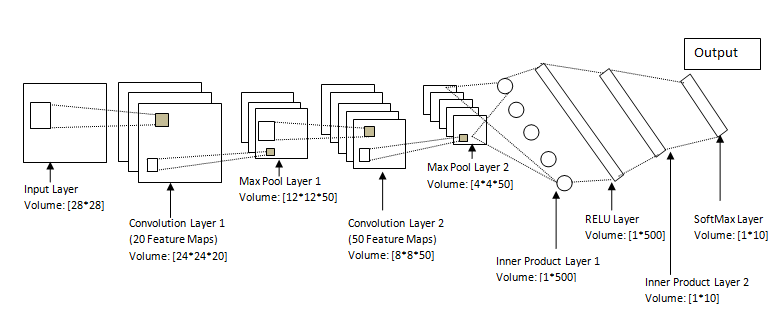
\includegraphics[scale=0.8]{figures/lenet5.PNG}
\caption{Lenet Model for MNIST Data Set Classification}
\label{fig:Lenet Application}
\end{figure}
\subsubsection{Convolution Layer 1}\label{Convolution layer 1}
In this layer a set of filters are slided spatially on the image to perform a 2 dimensional convolution operation.The layer takes 1 image of $[28\times 28]$ size as input and yields an output vector of size $[24\times 24 \times 20]$ considering that 20 filters are applied. The filters matrices are of dimension $[5\times 5]$ and contain single precision float values. 

\noindent The $[5\times 5]$ filter values may have different values based on the features e.g. edge detected or features representing small objects or regions in  an image e.g. edges , color, lines etc. The convolution layer 1 produces 20 filters where each filter is a $[24\times 24]$ map. The maps are stacked one over the other to produce the output.
\subsubsection{Max Pool Layer 1}\label{Max Pool layer 1}
Max pool layer is generally placed between two convolution layers. It performs a down sampling operation along the spatial dimensions which helps in reduction of parameters and computations. 

It takes the output maps from convolution layer 1 and applies a max operation on each $[2\times 2]$ slice of input i.e. (maximum of 4 values) is taken with a sliding step of 2 resulting in reduction of image size per image as $[12\times 12]$, however the number of maps remain the same.

\noindent It takes input of size $w\times h\times d$ $[24\times 24\times 20]$

\noindent Uses two parameters window size(z) and step size(s)  (2,2)

\noindent Produces an output of volume: $w'= (w-z)/s+1$, $h'= (h-z)/s+1$ and $d'=d$
\subsubsection{Convolution Layer 2}\label{Convolution layer 2}
It performs a 2D convolution operation as referenced in \ref{Convolution layer 1} on output volume from max pool layer 1. It takes a volume of size $[12\times 12\times 20]$ as input and generates an output volume of size $[8\times 8\times 50]$, specifying 50 filters on the given input. The filter size used is same as in \ref{Convolution layer 1} i.e. $[5\times 5]$.
\subsubsection{Max Pool Layer 2}\label{Max Pool layer 2}
From the output of convolution layer 2, again a down sampling operation is performed and an output volume is generated which has a volume of $[4\times 4\times 50]$.
\subsubsection{Inner Product Layer 1}\label{Inner Product Layer 1}
It is a fully connected layer wherein the neurons have full connections to all the  activation maps of the previous layer. The fully connected layer is converted to a convolution layer i.e. the input volume of size $[4\times 4\times 50]$ is converted to an input of $[1\times 800]$ considering the layer has 800 bias. The output of inner product layer is $[1\times 500]$ volume, which  involves 500 1D convolution of two $[1\times 800]$ matrices.
\subsubsection{Relu Layer}\label{Relu Layer}
Relu layer applies an element wise activation function,i.e. if the output is less that 0, it will set it to 0. The output dimensions are same as input.
\subsubsection{Inner Product Layer 2}\label{Inner Product Layer 2}
The output of Relu Layer is processed with another fully connected layer with 500 filters, which yields an output $[1\times 10]$
It produces the class scores based on the digits 0-10 resulting in a output of size $[1\times 1\times 10]$.
\subsubsection{Soft Max Layer}\label{Soft Max Layer}
It produces output probabilities based on the class scores.

\vspace{0.25cm}
\noindent The most computationally intensive part in the above implementation is convolution operation.

\section{Fixed Point Mathematics Implementation:}
The 2 dimensional convolution operation performs a multiplication operation, and then the result of this multiplication is added to the output variable for the $[5\times 5]$ overlap region of the input image and filter.
Functions were written to implement the above three operations in fixed point.

\vspace{0.25cm}
\noindent \textbf{Float to Fixed Format Conversion:}

\vspace{0.25cm}
\noindent It is used to convert the initial input value and filter value in the fixed point format by using the methodology described in section \ref{2.5.3}. It uses the roundf() function from the C++ maths library, which computes the nearest integer value to the floating point argument.

\lstset { %
	language=C,
	backgroundcolor=\color{lightgray}, % set backgroundcolor
	%basicstyle=\footnotesize,% basic font setting
	basicstyle=\ttfamily\scriptsize,
	%\basicstyle=\ttfamily\scriptsize,
	keywordstyle=\color{blue}\ttfamily,
	stringstyle=\color{red}\ttfamily,
	commentstyle=\color{darkgray}\ttfamily,
	breaklines=true	
}
\lstset{framesep=-10pt, xleftmargin=-10pt}
\begin{lstlisting} [caption={Sample Code to Convert from Float to Fixed}
,label={listing:2}]
int convert(float num1)
{
     int c;
     float b;
     
     //Scale floating point variable num1 up by a factor 2^frac_len
     b=num1*(2^frac_len);
     
     //use the Round function in the math library of C++ 
     //to round the variable to nearest integer.
     c=roundf(b);
     
     return(c);
}
\end{lstlisting}



\vspace{0.25cm}
\noindent \textbf{Fixed Point Addition:}

\vspace{0.25cm}
\noindent In the 2 dimensional convolution operation, the input and filter are converted in same Q32.\textit{frac\_len} format. The addition is performed for two numbers in same Q format as described in section \ref{2.5.3}.

\lstset { %
	language=C,
	backgroundcolor=\color{lightgray}, % set backgroundcolor
	%basicstyle=\footnotesize,% basic font setting
	basicstyle=\ttfamily\scriptsize,
	%\basicstyle=\ttfamily\scriptsize,
	keywordstyle=\color{blue}\ttfamily,
	stringstyle=\color{red}\ttfamily,
	commentstyle=\color{darkgray}\ttfamily,
	breaklines=true	
}
\lstset{framesep=-10pt, xleftmargin=-10pt}
\begin{lstlisting}[caption={Sample Code for Fixed Addition},label={listing:3}]
float addition (float num1,float num2)
{
     int n1,n2;
     float temp_result;
  
     //Convert num1 and num2 to fixed point using the function convert
     //as given in section 4.2.3
     n1=convert(num1);
     n2=convert(num2);
  
     //Return the result of fixed point addition
     temp_result=n1+n2;
  
     return temp_result;
}
\end{lstlisting}



\noindent In the above sample, the numbers are converted to fixed point and the result of addition is returned in fixed point format. The result can be converted back to float by scaling with a factor of $2^{-frac\_len}$ or can be used as it is in case of successive fixed point addition.

\vspace{0.25cm}
\noindent \textbf{Fixed Point Multiplication:}

\vspace{0.25cm}
\noindent The 2 dimensional convolution performs is modified to perform a fixed point multiplication on two numbers in the same Q format as described in Listing \ref{listing:4}.
\noindent 

\lstset { %
	language=C,
	backgroundcolor=\color{lightgray}, % set backgroundcolor
	%basicstyle=\footnotesize,% basic font setting
	basicstyle=\ttfamily\scriptsize,
	%\basicstyle=\ttfamily\scriptsize,
	keywordstyle=\color{blue}\ttfamily,
	stringstyle=\color{red}\ttfamily,
	commentstyle=\color{darkgray}\ttfamily,
	breaklines=true	
}
\lstset{framesep=-10pt, xleftmargin=-10pt}
\begin{lstlisting}[caption={Sample Code for Fixed Multiplication},label={listing:4}]
float multiply(float num1,float num2)
{
     int temp;
     int n1,n2;
     float temp_result; 
     
     //Convert num1 and num2 to fixed point using the function convert
     //as given in section 4.2.3
     n1=convert(num1); 
     n2=convert(num2);
    
     //compute Fixed Point Multiplication
      temp=n1*n2;
      
     //adjust the result of fixed point multiplication
     //by scaling down with 2^frac_len
      temp_result=temp/(2^frac_len);
      
      return temp_result;
}
\end{lstlisting}


\noindent The above sample takes two floating point numbers as input and returns the result of multiplication in fixed point format. The extra scaling by a factor of $2^{-frac\_len}$ specific to the multiplication operation as described in section \ref{2.5.3} is already performed. To convert the result back to floating point representation, the result returned from the function should be scaled by a factor of $2^{-frac\_len}$.
\section{Introduction to Libfi}
Libfi is a free open source template based header based binary fixed point library for C++, intended to be used for hardware.
\subsection{Main Features}
The library offers various features like, customizable rounding and overflow handling modes etc.
\subsubsection{Fixed Data type}
The fixed point data type under the namespace \textit{Fi} takes 5 parameters.
\begin{enumerate}
\item
\textbf{W:} It represents the total word length in bits, including the sign bit. W must be less than or equal to 32, however it does not necessarily have to be a power of two.
\item
\textbf{F:} It represents the number of fractional bits. F Must be less than or equal to W.
\item
\textbf{S:} It represents the signedness of the resulting type. Values for S are: signed denoted by (Fi::SIGNED) and unsigned denoted by (Fi::UNSIGNED).
\item
\textbf{OF:} It specifies the overflow handling mode for the fixed point number. It defaults to wrap-around.The other overflow handling modes are described in \ref{Overflow Section}. 
\item
\textbf{R:} It specifies the rounding mode. It defaults to rounding towards zero. The other rounding modes are described in \ref{Rounding Modes Section}.
\end{enumerate}
\vspace{0.5cm}
\textbf{Example Representations}

Fi::Fixed\textless8, 4, Fi::SIGNED, Fi::Wrap\textgreater a("3.14");

defines a signed fixed point variable having word length 8, fractional length 4, with the overflow handler \textit{wrap} representing value 3.14.

\vspace{0.5cm}
Fi::Fixed\textless8, 4, Fi::UNSIGNED, Fi::Saturate\textgreater a("3.14");

defines an unsigned fixed point variable having word length 8 and fractional length 4, with the overflow handler \textit{saturate} representing value 3.14.

\noindent Multiple constructors of the class \textit{Fixed} allow creation of fixed objects from floating point numbers,strings representing fixed point number or from other fixed point objects.
It also allows creation of a fixed object from a raw binary value representing a fixed point number.
Various logical operations are implemented e.g. Bitwise AND, OR,Comparison,Shifting operations etc.
\subsubsection{Rounding Modes}\label{Rounding Modes Section}
The library offers various fixed point rounding modes each of which is implemented with a separate round function in structure variables defining the modes.
\begin{enumerate}
\item
\textbf{NearOdd:} A value is rounded towards the nearest value, except for ties which are settled towards the nearest odd value.

\noindent The input is the fixed point number to be rounded and the rounded value alongwith a -1(+1) indicating that positive(negative) numbers can decrease(increase) in value as a result of rounding or 0 if the input is zero is returned.
\item
\textbf{NearEven:} A value is rounded towards the nearest value except for ties which are settled towards the nearest even value.

\noindent The input is fixed point number to be rounded and the rounded value alongwith a -1(+1) indicating that positive(negative) numbers can decrease(increase) in value as a result of rounding, or 0 if the input is zero is returned.
\item
\textbf{Floor:} A value is rounded towards negative infinity which  is also known as floor or negative. It always assumes that bits representing the fractional length will be rounded away.

\noindent The input is fixed-point number to be rounded and it returns the rounded value and -1 indicating that numbers can increase in value as a result of rounding, or 0 if the input is 0.
\item
\textbf{Fix:} A value is rounded towards zero, which is also known as fix or away from infinity. As rounding to floor, it also assumes that FRACTION LENGTH bits will be rounded away.

\noindent The input here in is the Fixed-point number to be rounded. It returns The rounded value and -1 (+1) indicating that positive (negative) numbers can decrease (increase) in value as a result of rounding, or 0 if the input is zero.	
\item
\textbf{Classic:}A value is rounded(up or down) towards nearest value. Ties are rounded away from zero.

\noindent It takes the fixed point number to be rounded as input and returns the rounded value and -1(+1) indicating that positive(negative) numbers can decrease (increase) in value.

\item
\textbf{Ceil:} A value is rounded towards positive infinity. It assumes that bits representing the fractional length will be rounded away.

\noindent The input is fixed point number to be rounded and it returns the rounded value and 1 indicating that numbers can increase in value as a result of rounding,or 0 if the input is 0.
\end{enumerate}
\subsubsection{Overflow}\label{Overflow Section}
The library offers various modes to handle overflows as described below:
\begin{enumerate}
\item
\textbf{Wrap Around:} A wrap around(modulus) overflow handler. 

\noindent If overflow occurs, the assigned value is the original value modulo $2^{(W+1)}$.
The input is the integer representing a fixed-point number and the return value is the number after wrapping is applied.
\item
\textbf{Saturate:} A saturating overflow handler.

\noindent If overflow occurs, the assigned value is set to nearest representable value. The input is the integer representing a fixed-point number and the return value is the number after saturation is applied.
\item
\textbf{Throw:} Throws an exception when overflow occurs.

\noindent If positive overflow occurs, Fi::PositiveOverflow is thrown.

\noindent If negative overflow occurs, Fi::NegativeOverflow is thrown.

\noindent The input is the integer representing a fixed-point number and the number provided in throws std::overflow\_error is returned.
\item
\textbf{Undefined:} It is used if undefined behavior in the event of an overflow can be accepted. Currently, the only advantage of using this over other overflow handler is a minor speed improvement as it is optimized for speed, although the actual behavior depends on the compiler and underlying system.

\noindent It takes the integer representing a fixed-point number as input and returns the number or a warning that the programmer is willing to accept undefined behavior in the event of an overflow.
\end{enumerate}

\section{Integration of Libfi with Existing Implementation of MNIST Data Set Classification}
Before downloading the library, Opencv needs to be setup in Linux and the path should be setup using LD\_LIBRARY\_PATH.
The library can be downloaded from the git repository as mentioned in \ref{lib}. The header files referencing various functions of \textit{Libfi} as specified below:

\noindent "fi/Fixed.hpp"

\noindent "fi/overflow/Wrap.hpp"

\noindent need to be added in the main file of \textit{Lenet5} application code file.
\begin{itemize}
\item
\textbf{Libfi: Conversion from Float to Fixed}

\noindent Considering a float point variable "X", a corresponding fixed point variable with specified word length (WL) and fractional length (FL) can be defined as:

\hspace{3cm}Fi::Fixed\textless WL, FL, Fi::SIGNED\textgreater a(X);

\noindent Here "a" represents the converted value of a floating point variable X with word length (WL) out of which FL represents the number of bits for fractional part.
\item
\textbf{Libfi: Conversion from Fixed to Float}

\noindent Considering a fixed point variable "a", with word length (WL) and fractional length (FL), the corresponding floating point converted variable "X" can be defined as:

\hspace{3cm}X = a.toFloat();

\noindent Here "X" represents the converted value of a fixed point variable "a" with word length (WL) out of which FL represents the number of bits for fractional part.
\item
\textbf{Libfi: Fixed Point Multiplication Example}

\noindent Considering two fixed point variables "a" and "b" defined with a word length (WL) and fractional length (FL), a fixed point multiplication can be performed as:

\lstset { %
	language=C,
	backgroundcolor=\color{lightgray}, % set backgroundcolor
	%basicstyle=\footnotesize,% basic font setting
	basicstyle=\ttfamily\scriptsize,
	%\basicstyle=\ttfamily\scriptsize,
	keywordstyle=\color{blue}\ttfamily,
	stringstyle=\color{red}\ttfamily,
	commentstyle=\color{darkgray}\ttfamily,
	breaklines=true	
}
\lstset{framesep=-10pt, xleftmargin=-10pt}
\begin{lstlisting}[caption={Libfi:Fixed Point Multiplication Example Code Snippet},label={listing:5}]
//include Fixed Point Library files.
#include "fi/Fixed.hpp"
#include "fi/overflow/Wrap.hpp"
#include <iostream>

#define WL 8
#define FL 4

int main(int argc, char* argv[]) 
{
     //Define two fixed point variables a and b
     Fi::Fixed<WL, FL, Fi::SIGNED> a("3.14");
     Fi::Fixed<WL, FL, Fi::SIGNED> b("1.14");
  
     //Display the result of Fixed Point multiplication.
     std::cout << a*b << std::endl;
  
     return 0;
}
\end{lstlisting}




\end{itemize}
\noindent The code snippet in listing \ref{listing:5} is written referring to the examples given in \ref{lib}. In the above example a fixed point multiplication operation is performed on two fixed Point variables: "a" having the value 3.14 and "b" having the value 1.14, stored in fixed point format with a word length 8 and fractional length 4 and the result is displayed on screen. The corresponding result obtained is 3.5. By performing the multiplication in floating point the corresponding result is 3.5796. The difference in values because of the rounding off errors introduced by using fixed point format. 

\vspace{0.25cm}
The convolution layers 1 and 2 of the application use a function \textit{CustomFilter2D} which performs a two dimensional convolution in floating point data types, on the feature maps with a 5 * 5 kernel as described in section \ref{Convolution layer 1} and \ref{Convolution layer 2}. In the 2D convolution operation, multiply accumulate operation is performed on two 5*5 matrices. The overlapping numbers of two matrices are multiplied and then the result of the multiplication is accumulated to generate a value.

\vspace{0.25cm}
The two dimensional convolution function is modified such that, the inputs are first converted in fixed points, and the fixed point multiplication is computed and the result is converted back to float and accumulated in the floating variable. The sample code Snippet given in \ref{fig:Custom Filter 2d} describes the operation.


\lstset { %
	language=C,
	backgroundcolor=\color{lightgray}, % set backgroundcolor
	%basicstyle=\footnotesize,% basic font setting
	basicstyle=\ttfamily\scriptsize,
	%\basicstyle=\ttfamily\scriptsize,
	keywordstyle=\color{blue}\ttfamily,
	stringstyle=\color{red}\ttfamily,
	commentstyle=\color{darkgray}\ttfamily,
	breaklines=true	
}
\lstset{framesep=-10pt, xleftmargin=-10pt}
\begin{lstlisting}[caption={Two Dimensional Convolution Operation Code Snippet},label={listing:61}]

out.at<float>(r,c) = 0;

for(int i = 0; i < ker.rows; i++) {

  for(int j = 0; j < ker.cols; j++) {   
    
    //Define a fixed point variable "a"
    //to store the fixed point value of kernel
    Fi::Fixed<word_length, frac_length, Fi::SIGNED> a(ker.at<float>(i, j));
    
    //Define a fixed point variable "b" 
    //to store the fixed point value of Input
    Fi::Fixed<word_length, frac_length, Fi::SIGNED> b(input.at<float>(r+i, c+j));
    
    //Define a fixed point variable "temp1" 
    //to store the result of fixed point multiplication
    Fi::Fixed<word_length, frac_length, Fi::SIGNED> temp1(a*b);
    
    //the result is converted back to float and added to the output.
	out.at<float>(r,c) += temp1.toFloat();
	
	}
}
\end{lstlisting}

\vspace{0.25cm}
In the code,given in listing \ref{listing:6}
\begin{itemize}
\item
\textit{word\_length} and \textit{frac\_length} are two macros defined to represent the number of bits to represent fixed point word and the number of bits used to represent the fractional part.
\item
\textit{ker} is a 5*5 Matrix, which represents the weights.
\item
For each 5*5 matrix multiplication, fixed point variable \textit{"a"} stores the fixed point converted value corresponding to a floating point value of \textit{ker} at a point.
\item
Similarly fixed point variable \textit{"b"} stores the fixed point converted value corresponding to a floating point value of \textit{input} at a point.
\item
The variable \textit{"temp1"} stores the result of the fixed point multiplication of \textit{a} and \textit{b}.
\item 
The result stored in \textit{"temp1"} is converted back to float and accumulated in the floating value at a point represented by \textit{out}.
\item 
The entire multiplication is performed in signed multiplication with a default rounding and overflow handling mode.
\end{itemize}
\noindent The \textit{"Fi"} folder under the \textit{Libfi} library is copied in the folder containing the C++ references for the implementation of MNIST data set classification. Makefile is updated to include the path of \textit{Libfi}, under the \textit{CPPFLAGS} link to avoid the include errors. Another way is to update the include path in all source files of \textit{Libfi} library.


\lstset { %
	language=C,
	backgroundcolor=\color{lightgray}, % set backgroundcolor
	%basicstyle=\footnotesize,% basic font setting
	basicstyle=\ttfamily\scriptsize,
	%\basicstyle=\ttfamily\scriptsize,
	keywordstyle=\color{blue}\ttfamily,
	stringstyle=\color{red}\ttfamily,
	commentstyle=\color{darkgray}\ttfamily,
	breaklines=true	
}
\lstset{framesep=-10pt, xleftmargin=-10pt}
\begin{lstlisting}[caption={Changes to Makefile},label={listing:6}]
include ./sources.mk

exec=lenet_app

CC=g++

CPPFLAGS=CPPFLAGS= -g $(shell pkg-config --cflags opencv)\
          -I/usr/local/include/opencv2\
           -I./fi -I ./
           
LIBS= $(shell pkg-config --libs opencv) -lpapi 
\end{lstlisting}



\noindent The application can be build by running the \textit{"make all"} command in the command line, with \textit{cpp-ref} folder as the working directory.

\vspace{0.25cm}
\noindent To check the result of a single image classification, the following command should be executed:

\vspace{0.25cm}
./lenet\_app -m sample -i ../imgs/mnist\_test\_img\_0.pgm

\vspace{0.25cm}
\noindent Here \textit{mnist\_test\_img\_0.pgm} is the image name. The results can be tested for other user specified images also.

\vspace{0.25cm}
\noindent To test the library for whole dataset of 10000 images, the test images folder in the \textit{imgs} folder of the library should be expanded followed by the execution of the following command :

\vspace{0.25cm}
./lenet\_app -m test -f ../imgs/mnist\_test\_img\_list.csv -d ../imgs/mnist-testset

\vspace{0.25cm}
\noindent \textbf{Sample Output:} The sample output for the execution of entire test set is as shown in figure \ref{fig:output_mnist}.

\begin{figure}[!h]
\centering
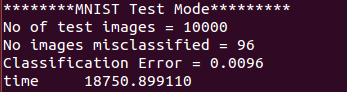
\includegraphics[scale=0.65]{figures/sample_output.png}
\caption{Sample Output for Test set of 10000 Images}
\label{fig:output_mnist}
\end{figure}
\noindent The existing implementation was simulated for combinations of word length and fractional length, keeping the word length as 32. The tests are run for MNIST test set comprising of 10000 images and the accuracy is computed in terms of number of images which are correctly classified.

\noindent The effect on accuracy of classification algorithm by varying the fixed point fractional length for word length of 32 and 16 are shown in table \ref{Results Fixed1} and \ref{Results Fixed2}.

\begin{table}[h]
\centering
\caption{Effect on Accuracy by varying the Fixed Point Fractional Length (Word Length 32).}
\label{Results Fixed1}
\begin{tabular}{||m{3cm}|m{1.5cm}|m{1.5cm}|m{1.5cm}|m{1.5cm}|m{1.5cm}|m{1.5cm}||}
\hline
\multirow{2}{*}{Metric} & \multirow{2}{*}{\parbox{1.5cm}{Floating Point Datatype}} & \multicolumn{5}{|c||}{ Fixed Point Fractional Length (Word Length 32)} \\[1.5ex]\cline{3-7}
& & 16bits&12 bits &8bits&4bits&2bits \\[1.5ex]
\hline
\hline
Number of images wrongly classified   & 95 &95 &95 &96 &567 &8865\\
\hline
Number of images correctly classified &9905&9905&9905&9904&9433&1135\\
\hline
Accuracy (\% of images correctly classified)&99.05\%&99.05\%&99.05\%&99.04\%&94.33\%&11.35\%\\
\hline
\end{tabular}

\end{table}

\begin{table}[!h]
\centering
\caption{Effect on Accuracy by varying the Fixed Point Fractional Length (Word Length 16).}
\label{Results Fixed2}
\begin{tabular}{||m{4cm}|m{2cm}|m{1.5cm}|m{1.5cm}|m{1.5cm}|m{1.5cm}||}
\hline
\multirow{2}{*}{Metric} &  \multicolumn{5}{|c||}{ Fixed Point Fractional Length (Word Length 16)} \\\cline{2-6}
& 16bits&12 bits &8bits&4bits&2bits \\
\hline
\hline
Exception& Positive Overflow &\multicolumn{4}{|c||}{-}\\
\hline
Number of images wrongly classified    &- &95 &96 &567 &8865\\
\hline
Number of images correctly classified  &- &9905&9904&9433&1135\\
\hline
Accuracy (\% of images correctly classified)&- &99.05\%&99.04\%&94.33\%&11.35\%\\
\hline
\end{tabular}

\end{table}
\noindent The effect of changing the fixed point bit-width on the accuracy can be seen in a more detailed manner from 
 \begin{figure}[!h]
\centering
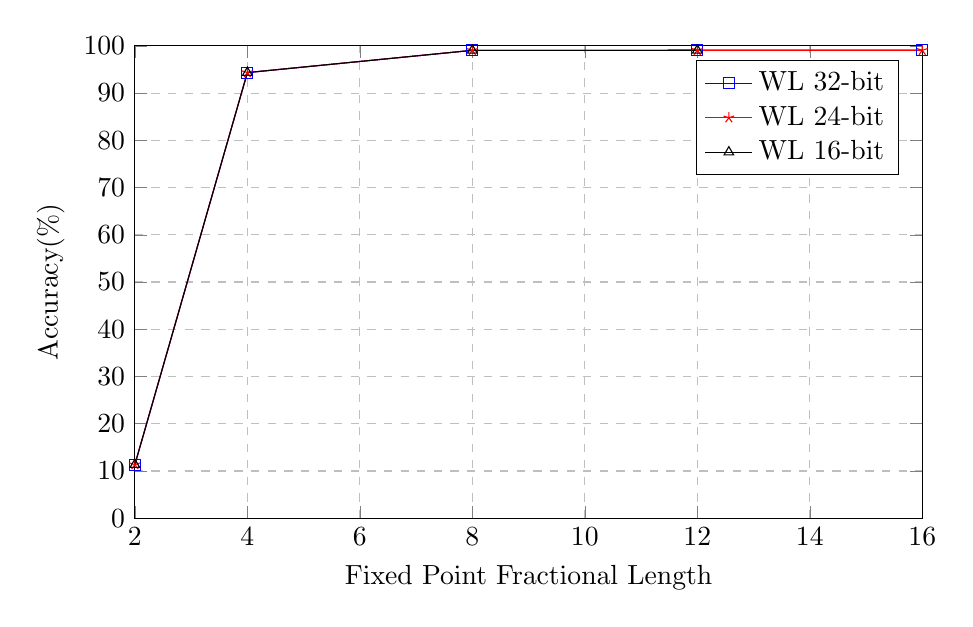
\begin{tikzpicture}
\begin{axis}[
scale only axis,
height=6cm,
width=10cm,
    xlabel={Fixed Point Fractional Length},
    ylabel={Accuracy(\%)},
    xmin=2, xmax=16,
    ymin=0, ymax=100,
    xtick={2,4,6,8,10,12,14,16},
    ytick={0,10,20,30,40,50,60,70,80,90,100},
    legend pos=north east,
    ymajorgrids=true,
    xmajorgrids=true,
    grid style=dashed,
]
\addplot[
    color=blue,
    mark=square,
    ]
    coordinates {
    (2,11.35)(4,94.33)(8,99.04)(12,99.05)(16,99.05)
    };
    \addlegendentry{WL 32-bit}
 \addplot[
    color=red,
    mark=star,
    ]
    coordinates {
    (2,11.35)(4,94.33)(8,99.04)(12,99.05)(16,99.05)
    };
   \addlegendentry{WL 24-bit}
  \addplot[
    color=black,
    mark=triangle,
    ]
    coordinates {
    (2,11.35)(4,94.33)(8,99.04)(12,99.05)
    };
   \addlegendentry{WL 16-bit}
\end{axis}
\end{tikzpicture}
\caption{Effect of varying the Fractional Length on Accuracy}
\label{fig:graph}
\end{figure}
\vspace{0.25cm}
\noindent It should be noted that for the given Lenet model, the accuracy increases with the increase in the number of fractional bits by keeping the fixed point word length constant. Because as the number of bits to store the fractional bits are increased, the system becomes more efficient to precisely store the values after the decimal point which in the course of algorithm after successive multiplications and additions may effect the reliability if not handled properly.

\vspace{0.25cm}
\noindent In this model, changing the word length also doesn't affect the readings, because the values are normalized and lie between 0 to 1. The result throws a positive overflow exception for Q16.16 combination of the fixed point which implies zero bits are supplied to store the integer part. So it cannot be simulated for Q16.16 format.

\vspace{0.25cm}
\noindent From the above results, it is verified that the accuracy for fixed point formats Q24.16 and Q32.16 is same as that of float.

\section{Introduction to HLS Arbitrary Precision Fixed Point Library}
The fixed point functions hardware can be implemented using the inbuilt class in Vivado HLS for arbitrary precision fixed point types in C++ which can be accessed by including the header file:

\hspace{3cm}\#include\textless ap\_fixed.h\textgreater

\noindent There are separate classes for signed an unsigned numbers e.g.

\hspace{3cm}ap\_fixed for Signed and 

\hspace{3cm}ap\_ufixed for Unsigned
\begin{itemize}
\item
\textbf{Fixed Point Representation:}
A fixed point number in the above class can be represented as:

ap\_[u]fixed\textless int W, int I, ap\_q\_mode Q, ap\_o\_mode O, ap\_sat\_bits N\textgreater;

In the above representation:
\begin{itemize}
\item
\textbf{W :} W represents the Word Length
\item
\textbf{I :} I represents the number of bits to represent integer part. This implies the number of bits used to represent the fractional part is W-I.
\item
\textbf{ap\_q\_mode Q :} It represents the quantization mode. There are multiple options supported by Vivado HLS for quantization modes as mentioned in table \ref{rounding}.
\begin{table}[!h]
\centering
\begin{tabular}{m{4cm} m{6cm}}
AP\_RND & Rounding to plus infinity\\
AP\_RND\_ZERO & Rounding to zero\\
AP\_RND\_MIN\_INF & Rounding to minus infinity\\
AP\_RND\_INF & Rounding to infinity\\
AP\_RND\_CONV & Convergent rounding\\
AP\_TRN (default) & Truncation\\
AP\_TRN\_ZERO & Truncation to zero
\end{tabular}
\caption{Vivado HLS Fixed Point Rounding Modes}
\label{rounding}
\end{table}
\item
\textbf{ ap\_o\_mode O :} It represents the overflow mode. Various overflow modes supported by Vivado HLS are as as mentioned in table \ref{overflow}.

\begin{table}[!h]
\centering
\begin{tabular}{m{4cm} m{6cm}}
AP\_SAT & Saturation\\
AP\_SAT\_ZERO& Saturation to zero\\
AP\_SAT\_SYM & Symmetrical saturation\\
AP\_WRAP & Wrap-around\\
AP\_WRAP\_SM&Sign magnitude wrap-around\\
\end{tabular}
\caption{Vivado HLS Fixed Point Overflow Modes}
\label{overflow}
\end{table}
\item
\textbf{ap\_sat\_bits N:} It represents the number of saturation bits. The saturation is executed based on the value of N.
\end{itemize}

\item
\textbf{Conversion from Fixed to other Datatypes:}
There are member functions to convert the fixed point variable to other datatypes e.g. float, double etc. 

\hspace{3cm} double ap\_[u]fixed::to\_double()

The above function can be used to convert a fixed point variable to double precision floating point.

\hspace{3cm} float ap\_[u]fixed::to\_float()

The above function can be used to convert a fixed point variable to single precision floating point.

\hspace{3cm} int ap\_[u]fixed::to\_int()

The above function can be used to convert a fixed point variable to integer.

\item
\textbf{Fixed Point Operations:} There are class methods which provide support for various mathematical operations.e.g. Addition, Subtraction, Multiplication. Other than this there are class methods that support various bit level operations also. e.g. Bit level logical operations, Shift operations etc.  
\end{itemize}
\section{Performance Estimates for 2D Convolution Operation}
The 2D convolution operation used in the deep neural network implementation \ref{papaa} was analyzed using Vivado HLS, with slight modifications based on fixed array sizes etc.
The input and kernel values from the \textit{lenet5app} were supplied for verifying the accuracy from simulation results. The function was tested for one 2D convolution operation which takes as input a [28*28] matrix and [5*5] kernel matrix and produces an output matrix of size [24*24].

\noindent The functions were implemented to perform the operation on floating point and fixed point data. The simulation results were verified for accuracy of computation. It was analyzed from the results from table \ref{Results Fixed}, that the accuracy of the implementation for Q(32-16) and Q(24-16) fixed point combinations is same as float.

\noindent The area estimates were realized from the synthesis report for ZC702 Zedboard and it was seen that the fixed point representation consumes significantly lesser number of resources compared to floating point and at the same time the number of cycles is also less for executing the operation as represented in table \ref{Table 4.2}.

\begin{table}[h]
\centering
\caption{Area Estimates Comparison for 2D Convolution Operation for Zedboard ZC702}
\label{Table 5.5}
\begin{tabular}{||m{4cm}|m{3cm}|m{2.5cm}|m{2.5cm}||}
\hline
Metric & Floating Point &  \multicolumn{2}{|c||} { Fixed Point}\\[1.5ex]\cline{3-4}
& & Q(32-16) & Q(24-16)\\[1.5ex]
\hline
\multicolumn{4}{||c||}{Timing Estimates}\\[1.5ex]
\hline
Clock (ns)&8.41 &8.47 & 8.47\\[1.5ex]
\hline
Latency(max)(Cycles) &165362 & 136562 &93362\\[1.5ex]
\hline
\multicolumn{4}{||c||}{Area Estimates}\\[1.5ex]
\hline
DSP48E &5 &4 & 2 \\[1.5ex]
\hline
LUT's & 933 &202 & 184\\[1.5ex]
\hline
Flip Flops & 556 & 164 &145\\[1.5ex]
\hline		
\end{tabular}

\end{table}
\noindent The results were analyzed for different fixed point word length and fractional length combinations and the effect on performance based on latency and resource utilization is studied which is described in the following graphs.


\begin{figure}[h]
\centering
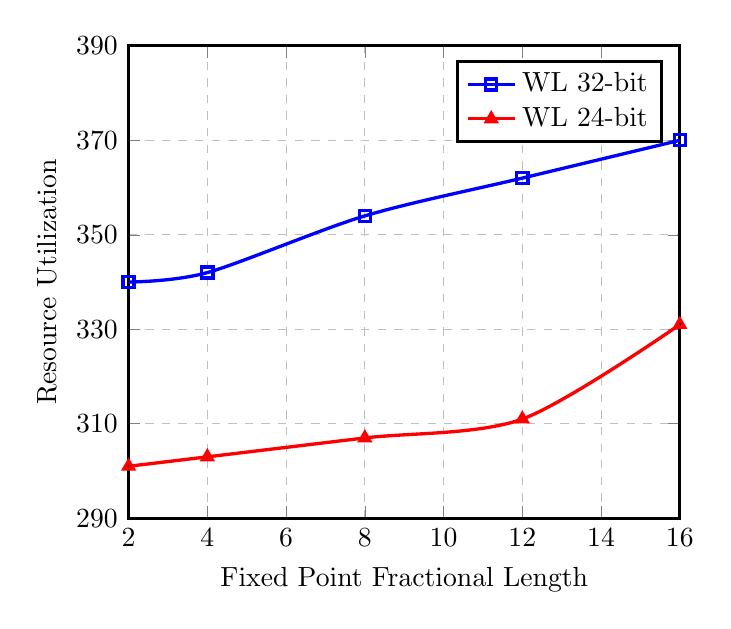
\begin{tikzpicture}
\begin{axis}[
scale only axis,
height=6cm,
width=7cm,
    xlabel={Fixed Point Fractional Length},
    ylabel={Resource Utilization},
    xmin=2, xmax=16,
    ymin=290, ymax=390,
    xtick={2,4,6,8,10,12,14,16},
    ytick={290,310,330,350,370,390},
    legend pos=north east,
    ymajorgrids=true,
    xmajorgrids=true,
    grid style=dashed,
    very thick
]
\addplot[
    color=blue,
    mark=square,
    smooth
    ]
    coordinates {
    (2,340)(4,342)(8,354)(12,362)(16,370)
    };
    \addlegendentry{WL 32-bit}
 \addplot[
    color=red,
    mark=triangle,
    smooth
    ]
    coordinates {
    (2,301)(4,303)(8,307)(12,311)(16,331)
    };
   \addlegendentry{WL 24-bit}
\end{axis}
\end{tikzpicture}
\caption{Effect of varying the Fractional Length on Resource Utilization}
\label{fig:5.5}
\end{figure}
\noindent It was observed that changing the fractional length as well as word length significantly reduces the number of resources used for the computation as can be seen from figure \ref{fig:5.5}.

\begin{figure}[!h]
\centering
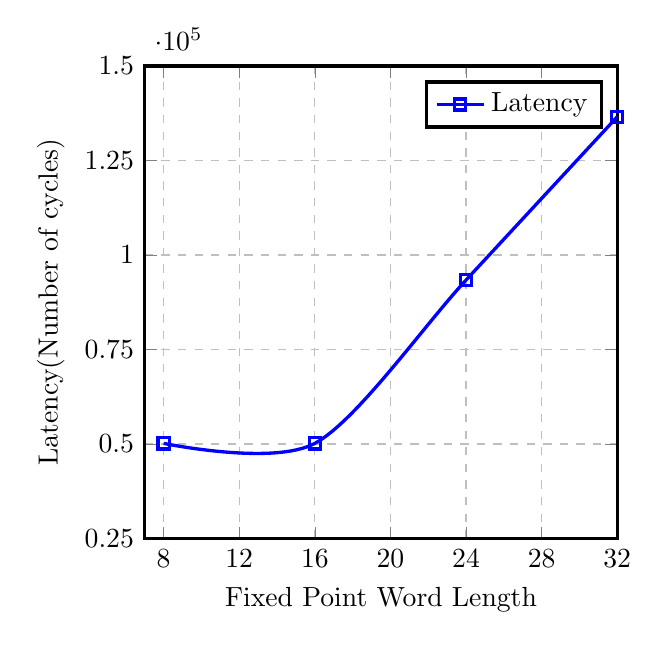
\begin{tikzpicture}
\begin{axis}[
scale only axis,
height=6cm,
width=6cm,
    xlabel={Fixed Point Word Length},
    ylabel={Latency(Number of cycles)},
    xmin=7, xmax=32,
    ymin=25000, ymax=150000,
    xtick={8,12,16,20,24,28,32},
    ytick={25000,50000,75000,100000,125000,150000},
    legend pos=north east,
    ymajorgrids=true,
    xmajorgrids=true,
    grid style=dashed,
    very thick
]
\addplot[
    color=blue,
    mark=square,
    smooth
    ]
    coordinates {
    (32,136562)(24,93362)(16,50162)(8,50162)
    };
    \addlegendentry{Latency}
\end{axis}
\end{tikzpicture}
\caption{Effect of varying the Fixed Point Word Length on Latency}
\label{fig:5.6}
\end{figure}
\noindent It was observed that changing the fractional length for a fixed word length doesn't have any impact on the latency for this algorithm. However the latency is improved by reducing the word length. The effect of varying the word Length on the latency is demonstrated in Figure \ref{fig:5.6}.

\noindent It should be noted that reducing the word length and fractional length at the same time have an adverse effect on the accuracy of the algorithm. So the trade offs must be analyzed before choosing the Q formats. Similarly changing the arithmetic blindly can affect the correctness of the scheme as we analyzed for FHEW. In the following chapter, the results and conclusions drawn from the experiments are demonstrated. 